%%%
%%% Document class and page properties
%%%

\documentclass[draft]{IIBproject}

% Set margin size
\usepackage[margin=2.5cm]{geometry}

% Set table of contents depth
\setcounter{tocdepth}{2}

%%%
%%% Standard packages in alphabetical order
%%%

% Use the AMS math package for special fonts such as mathbb (included in the amssymb package
% coming with ams math), inline text in equations, etc.
\usepackage{amsmath}
\usepackage{amssymb}

% Use the calc package for infix arithmetic
\usepackage{calc}

% Use the cleveref package for automatic formatting of reference
\usepackage{cleveref}
% Start all references with capital letters
\crefname{table}{Table}{Tables} 
\crefname{figure}{Figure}{Figures}
\crefname{section}{Section}{Sections}
% Completely redefine the equation reference format to remove parentheses around equations
\crefformat{equation}{#2Eq.~#1#3}
\crefrangeformat{equation}{Eqs.~#3#1#4 to~#5#2#6}
\crefmultiformat{equation}{Eqs.~#2#1#3}{ and~#2#1#3}{, #2#1#3}{ and~#2#1#3}

% Use BibTeX for bibliography management, use the hyperref package to include URLs in the entries
\usepackage{cite}
\usepackage{url}

% Color text
\usepackage{color}

% Use UTF-8 input encoding
\usepackage[utf8]{inputenc}

% Use the package for declaring paired delimiters
\usepackage{mathtools}

% Sets 1.5 line spacing
\usepackage{setspace}
\onehalfspacing

% Provides formatting of numbers (here used for thousands' separators)
\usepackage{siunitx}

% Use the tikz package for drawing
\usepackage{tikz}

\usetikzlibrary{decorations.pathreplacing}

% Provides robust spaces after commands
\usepackage{xspace}

%%%
%%% Commands
%%%

% Declare paired delimiters
\DeclarePairedDelimiter{\ceil}{\lceil}{\rceil}
\DeclarePairedDelimiter{\bracket}{(}{)}

% Define macros for correct spacing after abbreviations, source: http://tex.stackexchange.com/a/15017
\newcommand*{\eg}{e.g.\@\xspace}
\newcommand*{\ie}{i.e.\@\xspace}

% Abbreviations which can occur at the end of the sentence cannot duplicate the following dot
\makeatletter
\DeclareRobustCommand*{\AbbreviationWithDot}[1]{\@ifnextchar{.}{#1}{#1.\@\xspace}}
\DeclareRobustCommand*{\pmf}{\AbbreviationWithDot{p.m.f}}
\makeatother

% Placeholder for parts of the report to be finished later
\DeclareRobustCommand{\later}{\textcolor{red}{\textbf{(?)}}\@\xspace}

% Notes to be discussed with supervisor/thought about later
\DeclareRobustCommand{\noteSelf}[1]{\textcolor{red}{#1}}

% Ngram that cannot be broken over a line and uses emphasised font (i.e. usually is in italics)
\DeclareRobustCommand{\ngram}[1]{\emph{[#1]}}

% Macro for spelling out non-breaking (N-1)-grams and (N+1)-grams
\DeclareRobustCommand{\nmgram}{\mbox{$(N{-}1)$-gram}\@\xspace}
\DeclareRobustCommand{\nmgrams}{\mbox{$(N{-}1)$-grams}\@\xspace}
\DeclareRobustCommand{\npgram}{\mbox{$(N{+}1)$-gram}\@\xspace}
\DeclareRobustCommand{\npgrams}{\mbox{$(N{+}1)$-grams}\@\xspace}

%%%
%%% Drawing
%%%

% Define a new tikz style for drawings left-closed intervals: [i], notice that the heads are centred exactly on the start and end coordinates of the line
\usetikzlibrary{decorations.markings}
\tikzset{
    i/.style={
        shorten >=#1,
        decoration={
            markings,
            mark={ at position 0 with {\filldraw[solid] circle [radius=#1];} },
            mark={ at position 1 with {\draw[solid] circle [radius=#1];} }
        },
        postaction=decorate
    },
    i/.default=1.5pt
}

% Define macros for drawing a vertical interval, the arguments are always:
%	(#1,#2)	- start position
%	(0,#3)	- length vector
%	(#4,#5)	- beginning and end of the interval, normalised between 0 and 1
%	#6		- line style
%	#7		- position of the label ("left" or "right") if the interval is labelled
\newcommand{\interval}[6] {
	\draw[#6] [i] (#1,#2+#4*#3) -- (#1,#2+#5*#3);
}

\newcommand{\intervalTopLabel}[7] {
	\interval{#1}{#2}{#3}{#4}{#5}{#6}
	\node[#7] at (#1,#2+#5*#3) {\footnotesize #5};
}

\newcommand{\intervalBottomLabel}[7] {
	\interval{#1}{#2}{#3}{#4}{#5}{#6}
	\node[#7] at (#1,#2+#4*#3) {\footnotesize #4};
}

\newcommand{\intervalBothLabels}[7] {
	\intervalBottomLabel{#1}{#2}{#3}{#4}{#5}{#6}{#7}
	\node[#7] at (#1,#2+#5*#3) {\footnotesize #5};
}

%%%
%%% Document
%%%

\begin{document}

% Title page
\thispagestyle{empty}
\author{Konrad Komorowski (CHU)}
\title{Hiding Secrets in Plain Text}
\projectgroup{F}
\maketitle

% Summary and table of contents
\thispagestyle{empty}
\begin{abstract}
Lorem ipsum dolor sit amet, consectetur adipisicing elit, sed do eiusmod tempor incididunt ut labore et dolore magna aliqua. Ut enim ad minim veniam, quis nostrud exercitation ullamco laboris nisi ut aliquip ex ea commodo consequat. Duis aute irure dolor in reprehenderit in voluptate velit esse cillum dolore eu fugiat nulla pariatur. Excepteur sint occaecat cupidatat non proident, sunt in culpa qui officia deserunt mollit anim id est laborum.
\end{abstract}

\tableofcontents

% Contents
\pagestyle{plain}

\newpage
\section{Technical abstract}

Lorem ipsum.

\newpage
\section{Introduction}

Lorem ipsum.

\subsection{Aim}

\subsection{Overview of steganography}

\subsection{High level description of the stegosystem}

\newpage
\section{The interval algorithm}

The interval algorithm \cite{hanhoshi1997} provides a means of sampling from an arbitrary stochastic process (target) given an input sequence from a different arbitrary stochastic process (source). The algorithm is very similar to arithmetic coding -- it also uses successive refinements of the $[0,1)$ interval to map sequences.

The sequence mapping algorithm starts by mapping the empty sequence $[~]$ to the interval $[0,1)$. For any sequence, its interval is partitioned into subintervals corresponding to the sequence extended by a single term. The size of each interval is chosen to be proportional to the probability of the last term occurring given the preceding sequence. The order of the subintervals does not matter, but needs to be consistent if reverse mapping from an interval to a sequence is to be performed. By the chain rule of probability, the size of the resulting interval is equal to the probability of observing its sequence. Consequently, only sequences of non-zero probability can be mapped. For a more detailed overview of arithmetic coding see \cite{coverthomas:sfecoding}.

The interval algorithm works by continuously mapping the observed input sequence to successive intervals defined by the stochastic model of the source. In parallel, the intervals are reverse mapped to an output sequence according to the stochastic model of the target. Terms of the output sequence can be generated as long as its interval is a superinterval of the input sequence interval. See \cref{fig:interval_algorithm} for an example of the procedure.

\begin{figure}[h]
	\centering

	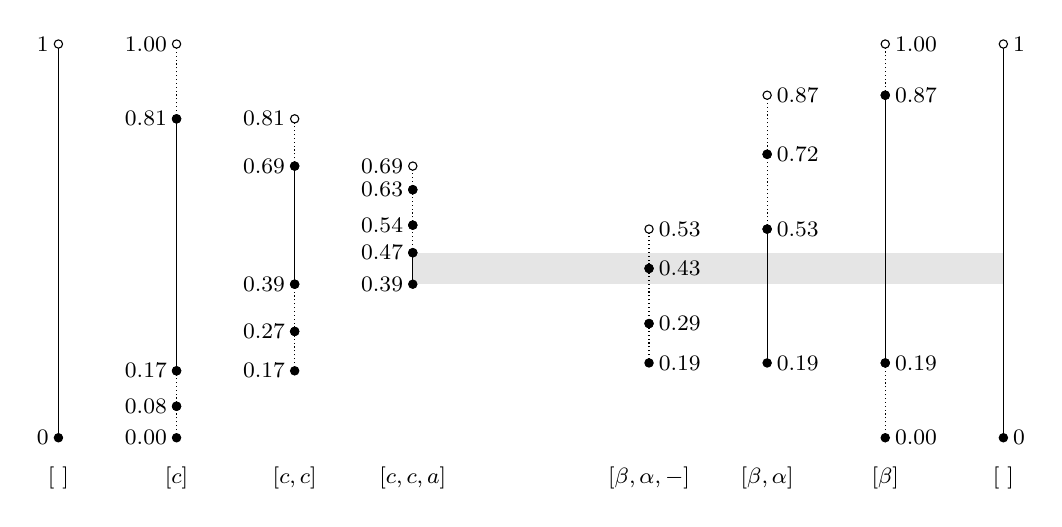
\begin{tikzpicture}[scale=0.05]
		% Final interval range
		\fill [opacity=0.1] (-30,0.39*100) rectangle (120,0.47*100);

		% Input side
		\intervalBothLabels{-120}{0}{100}{0}{1}{solid}{left}
		\node[below] at (-120,-5) {\footnotesize $[~]$};

		\intervalBothLabels{-90}{0}{100}{0.81}{1.00}{densely dotted}{left}
		\intervalBottomLabel{-90}{0}{100}{0.17}{0.81}{solid}{left}
		\intervalBottomLabel{-90}{0}{100}{0.08}{0.17}{densely dotted}{left}
		\intervalBottomLabel{-90}{0}{100}{0.00}{0.08}{densely dotted}{left}
		\node[below] at (-90,-5) {\footnotesize $[c]$};

		\intervalBothLabels{-60}{0}{100}{0.69}{0.81}{densely dotted}{left}
		\intervalBottomLabel{-60}{0}{100}{0.39}{0.69}{solid}{left}
		\intervalBottomLabel{-60}{0}{100}{0.27}{0.39}{densely dotted}{left}
		\intervalBottomLabel{-60}{0}{100}{0.17}{0.27}{densely dotted}{left}
		\node[below] at (-60,-5) {\footnotesize $[c,c]$};

		\intervalBottomLabel{-30}{0}{100}{0.39}{0.47}{solid}{left}
		\intervalBottomLabel{-30}{0}{100}{0.47}{0.54}{densely dotted}{left}
		\intervalBottomLabel{-30}{0}{100}{0.54}{0.63}{densely dotted}{left}
		\intervalBothLabels{-30}{0}{100}{0.63}{0.69}{densely dotted}{left}
		\node[below] at (-30,-5) {\footnotesize $[c,c,a]$};

		% Output side
		\intervalBothLabels{120}{0}{100}{0}{1}{solid}{right}
		\node[below] at (120,-5) {\footnotesize $[~]$};

		\intervalBothLabels{90}{0}{100}{0.87}{1.00}{densely dotted}{right}
		\intervalBottomLabel{90}{0}{100}{0.19}{0.87}{solid}{right}
		\intervalBottomLabel{90}{0}{100}{0.00}{0.19}{densely dotted}{right}
		\node[below] at (90,-5) {\footnotesize $[\beta]$};

		\intervalBothLabels{60}{0}{100}{0.72}{0.87}{densely dotted}{right}
		\intervalBottomLabel{60}{0}{100}{0.53}{0.72}{densely dotted}{right}
		\intervalBottomLabel{60}{0}{100}{0.19}{0.53}{solid}{right}
		\node[below] at (60,-5) {\footnotesize $[\beta,\alpha]$};

		\intervalBothLabels{30}{0}{100}{0.43}{0.53}{densely dotted}{right}
		\intervalBottomLabel{30}{0}{100}{0.29}{0.43}{densely dotted}{right}
		\intervalBottomLabel{30}{0}{100}{0.19}{0.29}{densely dotted}{right}
		\node[below] at (30,-5) {\footnotesize $[\beta,\alpha,-]$};

	\end{tikzpicture}

	\caption{\label{fig:interval_algorithm}Example run of the interval algorithm. The source returns symbols over the alphabet $\{a,b,c,d\}$, the target -- $\{\alpha,\beta,\gamma\}$. On the left, an input sequence $[c,c,a]$ from the source process gets mapped to $[0.39,0.47)$. On the right, this interval allows to generate up to 2 terms of an output sequence from the target process, \ie $[\beta,\alpha]$, which corresponds to $[0.19,0.53)$. Note that it is not possible to generate more terms of the output sequence, as neither $[0.19,0.29)$ nor $[0.29,0.43)$ nor $[0.43,0.53)$ is a superinterval of $[0.39,0.47)$.}

\end{figure}

\newpage
\section{Statistical natural language models}
\label{sec:snlm}

I will introduce basic principles of statistical natural language models. I will start by interpreting text as the output of a stochastic process and then apply approximations to make evaluating sentence probabilities computationally tractable. This section is mainly a review of \cite{4f11:statistical_language_models, 4f11:smt_systems, coursera:nlp}.

\subsection{Text as the output of a stochastic process}

A string $\mathbf w$ can be written as a sequence of $L$ \emph{tokens} $\mathbf w = [ w_1, \dots, w_L ] \equiv w_1^L$. Tokens are atomic elements of text such as words or punctuation marks. $w_l$ corresponds to the index of the token; for $V$ distinct tokens it takes values in $\{1, \dots, V\}$. $\mathbf w$ can be regarded as a realisation of an $L$-dimensional vector $\mathbf W$ of jointly distributed random variables $W_l$. According to the chain rule of probability, we can factorise $P(\mathbf w)$ as follows

\begin{equation}
\label{eq:exact_string_probability}
P(\mathbf w) = \prod_{l=1}^{L} P( w_l | w_1^{l-1} ) .
\end{equation}

Even though \cref{eq:exact_string_probability} gives a convenient formulation of language as a stochastic process, it is computationally intractable. If the conditional probabilities are stored in tables, the conditional probability table of the $l$th token has $V^l$ entries. Total size of all tables becomes prohibitively large for even small $L$.

\subsection{$N$-gram language models}

The usual solution is to restrict the size of the context to $N{-}1$ previous tokens, resulting in an approximate $N$-gram language model

\begin{equation}
\label{eq:ngram_string_probability}
P(\mathbf w) \approx P_{\text{$N$-gram}}(\mathbf w) \equiv \prod_{l=1}^{L} P( w_l | w_{l-N+1}^{l-1} ).
\end{equation}

\subsection{Estimating ML parameters}

The ML (maximum likelihood) estimate of conditional probability of $w_l$ in an $N$-gram model is

\begin{equation}
\label{eq:ml_conditional_token_probability}
\hat P( w_l | w_{l-N+1}^{l-1} ) = \frac {f(w_{l-N+1}^l)} {f(w_{l-N+1}^{l-1})},
\end{equation}

where $f(\cdot)$ is the number of occurrences of a particular sequence of tokens in training data.

A problem with \cref{eq:ml_conditional_token_probability} is that most $N$-gram counts will be zero. For example, a $5$-gram model with $V \approx 10^6$ will have $V^N \approx \left( 10^6 \right)^5 = 10^{30}$ distinct $N$-grams. For every possible $5$-gram sequence to occur at least once, training data would need to consist of more than $10^{30}$ tokens. Google Books $N$-gram Corpus \cite{googlengrams2011}, currently the largest available dataset, is based on $4.7 \times 10^{8}$ tokens. As a result, a large number of grammatically correct sentences will have zero probability.

\subsection{Limiting corpus size, discounting and back-off}

A standard way of dealing with this problem is to introduce \emph{discounting} and \emph{back-off} to the model. In addition, $N$-grams with counts below a threshold $C$ are sometimes discarded from the corpus to conserve storage space. The conditional distribution of the $l$th token becomes

\begin{equation}
	\label{eq:conditional_token_probability_with_backoff}
	P( w_l | w_{l-N+1}^{l-1} ) =
	\begin{cases}
		d (w_{l-N+1}^l) ~ \frac {f\left(w_{l-N+1}^l \right)} {f\left(w_{l-N+1}^{l-1} \right)} & \text{if $f(w_{l-N+1}^l) \ge C$},\\
		\alpha (w_{l-N+1}^l) ~ P( w_l | w_{l-N+2}^{l-1} ) & \text{otherwise},
	\end{cases}
\end{equation}

where $d(\cdot)$ and $\alpha(\cdot)$ return the discount and back-off weights -- scaling factors used to ensure that \cref{eq:conditional_token_probability_with_backoff} gives a valid \pmf. Intuitively, they reduce the mass assigned to observed $N$-grams to make space for estimates of order $N{-}1$ and lower.

$d(\cdot)$ and $\alpha(\cdot)$ are hard to choose or compute -- there exist many different schemes motivated by linguistics and statistics. Examples include Good-Turing smoothing \cite{good1953}, Kneser-Ney smoothing \cite{kneserney1995}, or stupid back-off \cite{brants2007} -- all exhibit various levels of complexity. In addition, the last does not even return a valid \pmf, but this is judged acceptable for strictly scoring applications.

\newpage
\section{Processing and storing $N$-gram counts}

I have shown that under certain assumptions $N$-gram counts are a sufficient statistic needed to evaluate probabilities of natural language text. In this section I will describe processing and efficient storage of these counts.

I will first describe two sources of data that I investigated, Google Books $N$-gram Corpus and Corpus of Contemporary American English $N$-grams, motivating why I chose the former. I will then explain in detail processing required to make the $N$-gram counts corpus fit for a steganographic application.

Firstly, all $N$-grams that contain digits are removed from the corpus. This is because they are frequently associated with illegible fragments of text from various data tables. Token strings of the remaining $N$-grams are then transliterated from Unicode to 7-bit ASCII, followed by conversion to lowercase letters and filtering only a set of allowed characters. The desired result is to remove noise from the system and make token representations unambiguous. Following this, extended tokens like \ngram{it's} are split into multiple base tokens such as \ngram{it}, \ngram{'} and \ngram{s}. The aim is to ensure that a fragment of text has a unique sequence of corresponding tokens. An algorithm to induce counts of base tokens from counts of the extended tokens is illustrated. Lastly, a procedure to enforce the $N$-gram counts to be self-consistent is described. Counts self-consistency is required by the language model from the next section.

Final counts are stored using a binary storage format referred to as BinDB (binary database). BinDB files store $N$-grams in sorted order, what allows efficient binary search. Additionally, $N$-grams with a common prefix will be adjacent to each other.

\subsection{Sources of natural language statistical data}

\subsubsection{Google Books $N$-gram Corpus}

Google has published $N$-gram counts, for up to $N=5$, compiled from 4.5 million scanned English books that contain 468 million tokens \cite{googlengrams2011, lin2012paper}. Their counts are given over different years when the books were published. The cutoff for including an $N$-gram in the corpus is $40$ occurrences in all books over all years. The tokens include part-of-speech (POS) annotations for words.

Currently, there are two version of the corpus -- 2009 and 2012. $N$-grams from the second version include special tokens for the beginning and end of sentence markers and cannot span sentence boundaries. Sentences across pages are detected. The first version of the corpus does not have these markers and the $N$-grams can span multiple sentences, but not pages. For higher accuracy, I decided to use the newer corpus.

All $N$-grams are stored in plain text files in the following format:

\centerline{\texttt{ngram TAB year TAB match\_count TAB volume\_count NEWLINE}}

where the \texttt{ngram} field is tab-separated into $N$ token strings. \texttt{match\_count} gives the total number of occurrences of an $N$-gram in the whole corpus in a given year, and \texttt{volume\_count} tells in how many different books published in that year it was found.

Tokens can be pure plain text strings (\eg \texttt{burnt}), part-of-speech annotated strings (\eg \texttt{burnt\_VERB}) or just the POS tags (\eg \texttt{\_VERB\_}). The first case corresponds to the existence of a particular string regardless of its role in the sentence. These are then broken down into finer categories, which indicate the syntactic role of a particular token, producing POS-annotated strings. The last class of tokens allows us to answer more general questions, for example the count of \mbox{\texttt{he \_VERB\_}} tells us how many times the word \emph{he} is followed by any verb.

$N$-grams up to $N=3$ are constructed by mixing tokens of all kinds, making it possible to ask all possible questions about counts. For $N \ge 4$ there are some restrictions to limit combinatorial explosion of corpus size. But $N$-grams consisting of plain string tokens are always available for every order $N$.

In the stegosystem, we need to have no ambiguity as to the identity of the token. Outputting text with POS tags would be a very strong indication that the system was used to generate it, so would compromise innocuousness. As a result, we are forced to use the unannotated tokens. Thus we will operate on a less precise language model, where sequences of tokens are less likely to be grammatically correct.

\subsubsection{Corpus of Contemporary American English $N$-grams}

Mark Davies has compiled $N$-gram frequencies \cite{web:byu_ngrams} from the Corpus of Contemporary American English (COCA) \cite{coca2010}. COCA is based on 0.2 million texts that contain a total of 440 million tokens. The tokens include POS-annotated words or punctuation, but not sentence markers. Free version of the database contains 1 million most frequent $N$-grams for each $N$ up to 5. Paid version has no cutoff and has counts of all $N$-grams up to $N=4$.

Prior to processing Google Books data, I experimented with using the free version of COCA $N$-grams to create the language model. I finally decided to use the Google Books $N$-grams Corpus because of free access its full version and the fact that it contains counts up to $N=5$. Since COCA $N$-grams are not a part of the final outcome of the project, I will not be discussing in detail their processing and storage.

\subsection{Normalising tokens}

\subsubsection{Discarding $N$-grams containing digits}

The Google Books $N$-gram Corpus is based on many books, some of which include data tables. As a result, they contain a large number of $N$-grams consisting of just numbers and punctuation marks. Randomly generated text would sometimes include long sections of those. To avoid such a possibility, I decided to create a second version of the corpus where $N$-grams containing digits are discarded. The trade-off is that most dates like \emph{July~4, 1776} will no longer be a part of the language.

\subsubsection{Normalising tokens using the \texttt{unidecode} package}

Google Books team made the best effort to represent each character of a token as precisely as possible using the full range of Unicode characters. This may be problematic -- equivalent words may be written in multiple ways and some characters will be impossible to represent using certain media. In addition, interpretation of text will be very sensitive to encoding -- not only the character glyph, but its underlying Unicode representation will matter.

To mitigate these problems, the tokens are \emph{normalised}. The first step is to transliterate Unicode text into plain 7-bit ASCII using using the \texttt{unidecode} Python package \cite{lib:unidecode}. Following this, uppercase letters are converted to lowercase. Finally, the tokens are filtered to contain only characters from \cref{tab:normal_characters}.

\begin{table}[h]
	\centering
	\begin{tabular}{r | l}
	\multicolumn{1}{c |}{class} & \multicolumn{1}{c}{characters} \\
	\hline
	lowercase letters & \texttt{\footnotesize a b c d e f g h i j k l m n o p q r s t u v w x y z} \\
	digits & \texttt{\footnotesize 0 1 2 3 4 5 6 7 8 9} \\
	punctuation & \texttt{\footnotesize !\ "\ \#\ \$\ \%\ \&\ \'\ (\ )\ *\ +\ ,\ -\ .\ /\ :\ ;\ <\ =\ >\ ?\ @\ [\ \textbackslash\ ]\ \textasciicircum\ \_\ `\ \{\ |\ \}\ \textasciitilde}
	\end{tabular}
	\caption{\label{tab:normal_characters}Characters that can be a part of a normalised token.}
\end{table}

\cref{tab:normalisation_examples} shows examples of the normalisation procedure. Note that some tokens are normalised to an empty string -- this is not a problem since they will be simply ignored. However, \texttt{unidecode} sometimes transliterates special symbols to a question mark in square brackets, \ie \emph{[?]}. Ideally these situations should be detected and handled using an empty string, but they are rare enough not to affect the model in a considerable way if ignored. Also, despite being understandable, the normalisation of \emph{Universitätsstraße} is strictly wrong -- in German \emph{ä} should be transliterated to \emph{ae}\cite{standard:din5007v2}.

\begin{table}[h]
	\centering
	\begin{tabular}{c | c}
	unnormalised & normalised \\
	\hline
	Ægean & aegean \\
	œuvre & oeuvre \\
	\textsterling & ps \\
	Universitätsstraße & universitatsstrasse \\
	\copyright & (c) \\
	$\leq$ & \textless= \\
	$\clubsuit$ & \emph{empty string} \\
	$\preccurlyeq$ & [?]
	\end{tabular}
	\caption{\label{tab:normalisation_examples}Example tokens containing special characters before and after normalisation.}
\end{table}

\subsubsection{Exploding tokens by punctuation}
\label{sec:exploding_tokens}

\cref{tab:its_ngrams} shows counts of three chosen $N$-grams: \ngram{it's}, \ngram{it 's} and \ngram{it ' s}. Even though they consist of respectively 1, 2 and 3 tokens, in plain text they all should be formatted in the same way -- as \emph{it's}. This introduces ambiguity -- if we observe \emph{it's} we do not know if we should interpret it as a 1-, 2- or 3-gram.

\begin{table}[h]
	\centering
	\begin{tabular}{c | c | c | c | r}
	$N$ & $w_1$ & $w_2$ & $w_3$ & \multicolumn{1}{c}{$f(w_1^N)$} \\
	\hline
	1 & it's & & & \num{37406} \\
	2 & it & 's & & \num{78658875} \\
	3 & it & ' & s & \num{7060268}
	\end{tabular}
	\caption{\label{tab:its_ngrams}Ways in which \emph{it's} is stored in the Google Books $N$-gram Corpus (after normalisation).}
\end{table}

The corpus needs to be processed in a way such that all entries from \cref{tab:its_ngrams} are absorbed into a single $N$-gram. It can be achieved through \emph{exploding tokens by punctuation}. Let us classify tokens into two groups: \emph{extended tokens} and \emph{base tokens}. A base token can consist of any number of lowercase letters and digits (\ie alphanumeric characters) or a single punctuation mark. An extended token is a concatenation of base tokens, where two alphanumeric base tokens cannot appear next to each other. Exploding a token by punctuation is defined as finding the corresponding base token sequence of an extended token.

\begin{table}[h]
	\centering
	\begin{tabular}{c | c}
	extended token & base tokens \\
	\hline
	e.g. & e\ .\ g\ . \\
	it's & it\ '\ s \\
	mr. & mr\ . \\
	yesterday). & yesterday\ )\ . \\
	"great" & "\ great\ " \\
	... & .\ .\ . \\
	\textless= & \textless\ =
	\end{tabular}
	\caption{\label{tab:extended_tokens}Example extended tokens with their corresponding base token sequences.}
\end{table}

If we explode tokens in \cref{tab:its_ngrams}, all $N$-grams will correspond to the same sequence of base tokens: \ngram{it ' s}. More generally, any phonological word that can be ambiguously split into multiple tokens because of internal punctuation can be uniquely identified by its sequence of base tokens.

\subsection{Induced counts of base $N$-grams}

The Google Books $N$-gram Corpus supplies counts of 1- to 5-grams of unnormalised extended tokens. In order to be able to interpret and generate plain text in an unambiguous way, we need to operate on tokens that are normalised and exploded by punctuation. We know how to apply normalisation and explosion to plain text, but we do not know the statistics of the resulting tokens -- we do not have $N$-gram counts from training data processed in this way. We need to induce such counts from the Google Books $N$-gram Corpus.

\subsubsection{Extended and base $N$-grams}

\emph{Extended $N$-gram} will refer to a sequence of $N$ unnormalised extended tokens (as stored in the Google Books $N$-gram Corpus). \emph{Base $N$-gram} will refer to a sequence of $N$ normalised base tokens (counts of which we wish to know). See \cref{fig:extended_and_base_ngrams} for examples of both.

% 	ngramMark: draw a horizontal segment signifying ngram boundary
%
%	#1	- start position of the ngram
%	#2	- end position of the ngram
%	#3	- vertical coordinate of the mark
\newcommand{\ngramMark}[3] {
	%\filldraw (#1,#3) circle (3.5pt);
	\draw [very thick] (#1,#3)--(#2,#3);
	%\filldraw (#2,#3) circle (3.5pt);
	% Alternative style with arrows at the end
	%\draw [<->] (#1,#3)--(#2,#3);
}

% 	extendedTokenDelimiter: draw a delimiter between extended tokens
%
%	#1	- horizontal coordinate between extended tokens
\newcommand{\extendedTokenDelimiter}[1] {
	\draw (#1,-19)--(#1,14.5);
}

% 	baseTokenDelimiter: draw a delimiter between base tokens within an extended token
%
%	#1	- horizontal coordinate between base tokens
\newcommand{\baseTokenDelimiter}[1] {
	\draw [dotted] (#1,-19)--(#1,14.5);
}

%	ngramsLabel: label a class of ngram markers
%
%	#1	- vertical coordinate of the lowest marker
%	#2	- vertical coordinate of the highest marker
\newcommand{\ngramsLabel}[3] {
	\draw [decorate,decoration={brace,amplitude=2.5pt,raise=2.5pt}] (-1,#1) -- (-1,#2) node [midway,left,xshift=-5pt] {#3};
}

\begin{figure}[h]
\centering
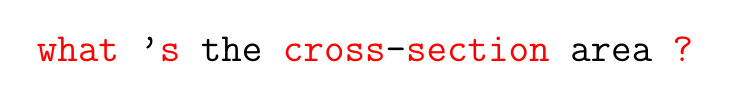
\begin{tikzpicture}[scale=0.312]

	\node [right] at (-0.45,0) {\Large \texttt{\textcolor{red}{what} '\textcolor{red}{s} the \textcolor{red}{cross}-\textcolor{red}{section} area \textcolor{red}{?}}};
%	\node [right] at (-0.45,0) {\Large \texttt{\textcolor{red}{what 's the cross-section area ?}}};

	% Extended token delimiters
	\extendedTokenDelimiter{-0.5}
	\extendedTokenDelimiter{4.5}
	\extendedTokenDelimiter{7.5}
	\extendedTokenDelimiter{11.5}
	\extendedTokenDelimiter{25.5}
	\extendedTokenDelimiter{30.5}
	\extendedTokenDelimiter{32.5}

	% Base token delimiters
	\baseTokenDelimiter{6}
	\baseTokenDelimiter{17}
	\baseTokenDelimiter{18}

	% Extended 1-grams
	\ngramMark{-0.5}{4.5}{3}
	\ngramMark{4.5}{7.5}{3.5}
	\ngramMark{7.5}{11.5}{4}
	\ngramMark{11.5}{25.5}{4.5}
	\ngramMark{25.5}{30.5}{5}
	\ngramMark{30.5}{32.5}{5.5}

	\ngramsLabel{3}{5.5}{Extended 1-grams}

	% Extended 2-grams
	\ngramMark{-0.5}{7.5}{7.5}
	\ngramMark{4.5}{11.5}{8}
	\ngramMark{7.5}{25.5}{8.5}
	\ngramMark{11.5}{30.5}{9}
	\ngramMark{25.5}{32.5}{9.5}

	\ngramsLabel{7.5}{9.5}{Extended 2-grams}

	% Extended 3-grams
	\ngramMark{-0.5}{11.5}{11.5}
	\ngramMark{4.5}{25.5}{12}
	\ngramMark{7.5}{30.5}{12.5}
	\ngramMark{11.5}{32.5}{13}

	\ngramsLabel{11.5}{13}{Extended 3-grams}

	% Base 1-grams
	\ngramMark{-0.5}{4.5}{-3}
	\ngramMark{4.5}{6}{-3.5}
	\ngramMark{6}{7.5}{-4}
	\ngramMark{7.5}{11.5}{-4.5}
	\ngramMark{11.5}{17}{-5}
	\ngramMark{17}{18}{-5.5}
	\ngramMark{18}{25.5}{-6}
	\ngramMark{25.5}{30.5}{-6.5}
	\ngramMark{30.5}{32.5}{-7}

	\ngramsLabel{-7}{-3}{Base 1-grams}

	% Base 2-grams
	\ngramMark{-0.5}{6}{-9}
	\ngramMark{4.5}{7.5}{-9.5}
	\ngramMark{6}{11.5}{-10}
	\ngramMark{7.5}{17}{-10.5}
	\ngramMark{11.5}{18}{-11}
	\ngramMark{17}{25.5}{-11.5}
	\ngramMark{18}{30.5}{-12}
	\ngramMark{25.5}{32.5}{-12.5}

	\ngramsLabel{-12.5}{-9}{Base 2-grams}

	% Base 3-grams
	\ngramMark{-0.5}{7.5}{-14.5}
	\ngramMark{4.5}{11.5}{-15}
	\ngramMark{6}{17}{-15.5}
	\ngramMark{7.5}{18}{-16}
	\ngramMark{11.5}{25.5}{-16.5}
	\ngramMark{17}{30.5}{-17}
	\ngramMark{18}{32.5}{-17.5}

	\ngramsLabel{-17.5}{-14.5}{Base 3-grams}

\end{tikzpicture}
\caption{\label{fig:extended_and_base_ngrams}Finding extended and base $N$-grams in the fragment of text \emph{what's the \mbox{cross-section} area?} Solid vertical lines denote boundaries between extended tokens, dotted vertical lines -- boundaries between base tokens. All $N$-grams up to $N=3$ are shown in the figure. Each is represented by a single thick horizontal segment. Extended $N$-grams are located above text, base $N$-grams -- below it.}
\end{figure}

Note that extended token boundaries are chosen by the Google Books team using a custom rule-based system \cite{lin2012thesis}, not necessarily in a way consistent for the same phonological word. \Cref{fig:extended_and_base_ngrams} shows an example way of how token boundaries could be found in a sentence. Base token boundaries are created using the algorithm from \cref{sec:exploding_tokens}.

\subsubsection{Inducing counts from extended 1-grams}

We know the counts of all extended $N$-grams up to a certain order and wish to know the counts of all base $N$-grams up to the same order. Both sets of counts are on the same text.

Looking at \cref{fig:extended_and_base_ngrams}, it is possible to state unique correspondence between extended 1-grams and some base $N$-grams. For example, the extended 1-gram \ngram{\mbox{cross-section}} coincides with and only with the set of base 1-grams \ngram{cross}, \ngram{-}, \ngram{section}, base 2-grams \ngram{cross -}, \ngram{- section} and base 3-gram \ngram{cross - section}. Let us call the elements of this set \emph{induced $N$-grams}. Formally, induced $N$-grams are base $N$-grams that can be identified in the base token sequence of an extended 1-gram.

Any time we observe counts of an extended 1-gram, we know that its induced $N$-grams occurred the same number of times. It is not a problem if we end up with multiple counts of the same induced $N$-gram. It means that this base $N$-gram occurs in many contexts and its counts need to be cumulated. Duplicates can come from the same extended 1-gram or different extended 1-grams. In the former case, \ngram{!!} gives \ngram{!} and \ngram{!}. In the latter, \ngram{mr.} gives \ngram{mr} and \ngram{.}, while \ngram{mrs.} gives \ngram{mrs} and \ngram{.} again.

\subsubsection{Inducing counts from extended $N$-grams ($N > 1$)}

Let us introduce more nomenclature. An \emph{extended $M$-gram} is a proper substring over the extended tokens of an extended $N$-gram. For example, the extended $N$-gram \ngram{'s the \mbox{cross-section}} has extended $M$-grams \ngram{'s}, \ngram{the}, \ngram{\mbox{cross-section}}, \ngram{'s the} and \ngram{the \mbox{cross-section}}.

Inducing counts from extended $N$-grams for $N>1$ is similar to the case when $N=1$. An equivalent sequence of base tokens has to be constructed as well, but \emph{not all} possible induced $N$-grams can be selected to be counted. If a base $N$-gram can be also induced from an extended $M$-gram, it \emph{cannot} be selected. If we did select it while processing the extended $N$-gram, it would be double counted -- we are guaranteed to come across its count again when processing the offending $M$-gram.

The above restriction can be easily stated in an equivalent way. A base $N$-gram induced from an extended $N$-gram has to contain at least one base token from the first and last extended tokens of the extended $N$-gram. This is how we ensure that it cannot be induced from an extended $M$-gram.

Using the example from the beginning of the section, \ngram{\underline{'s} the \mbox{\underline{cross-section}}} corresponds to the base token sequence \ngram{\underline{' s} the \underline{cross - section}}. The following induced $N$-grams can be selected from it: 3-gram \ngram{\underline{s} the \underline{cross}}, 4-grams \ngram{\underline{' s} the \underline{cross}}, \ngram{\underline{s} the \underline{cross -}} and 5-grams \ngram{\underline{' s} the \underline{cross -}}, \ngram{\underline{s} the \underline{cross - section}}. In all examples, base tokens that belong to the first or last extended token of the extended $N$-gram are underlined.

\subsection{Sentence delimiters}

Google Books $N$-grams contain \ngram{\_START\_} and \ngram{\_END\_} tokens to identify beginning and end of a sentence. If text is \emph{generated} using the language model, it will inevitably contain these tokens (for example any sequence will start with \ngram{\_START\_}). As a result some kind of convention needs to be adopted as to how sentence delimiters are identified in formatted output text. I decided that sentences will be delimited with multiple whitespace characters, for example a double space. I will return to this issue in the discussion section, as it has non-trivial consequences for practical application of the system.

\subsection{BinDB file format}

\noteSelf{Quickly describe the BinDB format -- binary storage of $N$-grams, format of each line, tokens are stored using their indices, $N$-grams are sorted.}

\subsection{Counts consistency}
\label{sec:counts_consistency}

\subsubsection{Definition}

$N$-grams are defined to be \emph{left counts consistent} if

\begin{equation}
\label{eq:left_counts_consistency}
\forall_{w_1^N} ~~ f(w_1^N) \ge \sum_{w_{N+1}} f(w_1^{N+1}),
\end{equation}

and \emph{right counts consistent} if

\begin{equation}
\label{eq:right_counts_consistency}
\forall_{w_1^N} ~~ f(w_1^N) \ge \sum_{w_0} f(w_0^N).
\end{equation}

$N$-grams are \emph{counts consistent} if they are both left and right counts consistent. If there is no cutoff for including an $N$-gram in the corpus, the equations become equalities.

\Cref{eq:left_counts_consistency,eq:right_counts_consistency} are easy to interpret. Left counts consistency ensures that if we add the counts of all \npgrams created by appending a token to the end of an $N$-gram, their sum will not be larger than the count of the $N$-gram. Right counts consistency is analogous. Obviously, $N$-grams that are correctly counted will be counts consistent.

\subsubsection{Ensuring counts consistency}

The Google Books $N$-grams Corpus is not counts consistent. This may be caused by a bug in the script that processed $N$-gram counts on-the-fly from Google servers. It skipped the last $N$-gram from each of the 2892 files that the corpus is split into. The corpus may also be inconsistent itself, for example due to the failure of some jobs during its distributed creation.

Counts consistency is assumed in some parts of the stegosystem, for example in $\beta{-}\gamma$ estimation in \cref{sec:beta_gamma_backoff}. Since inconsistencies are very rare (in the order of $10^3$ for the whole corpus of about $1.5 \times 10^9$ base $N$-grams), they can be forcefully corrected without visibly distorting information in the counts.

The highest order $N$-grams are asserted to be counts consistent, since there are no \npgrams to check with. In general, $N$-grams are made counts consistent in the following way:

\begin{enumerate}
\item \label{alg:cc_left_integration} \npgram counts are \emph{left integrated}. Last token is dropped from each \npgram to create a \emph{quasi}-$N$-gram. The counts of all identical \emph{quasi}-$N$-grams are cumulated.
\item \label{alg:cc_left_consistency} Left counts consistent $N$-grams are created by \emph{maximising} $N$-gram and \emph{quasi}-$N$-gram counts. Maximisation is performed as follows: both tables are simultaneously iterated over, starting from the first row. Whenever a \emph{quasi}-$N$-gram has a higher count than the same $N$-gram, the $N$-gram count is updated. If there is \emph{quasi}-$N$-gram without a corresponding $N$-gram, a new $N$-gram is created. Otherwise, the original $N$-grams are copied.
\item \label{alg:cc_full_consistency} Final counts consistent $N$-grams are created in a similar way. This time, \emph{right integrated} \npgrams are maximised with left counts consistent $N$-grams from the previous step.
\end{enumerate}

Steps \ref{alg:cc_left_consistency}-\ref{alg:cc_full_consistency} can be performed simultaneously, \ie jointly maximising all three tables of $N$-gram counts. In addition, since removing the last token does not change ordering, left integrated \npgrams can be created \emph{in place} -- identical \emph{quasi}-$N$-grams will be next to each other in the \npgrams table. However, creating right integrated \npgrams requires expensive sorting of the whole \emph{quasi}-$N$-grams table before cumulating them -- ordering is not preserved after removing the first token.

Creating count consistent of $N$-grams requires counts consistent \npgrams. So $N$-gram tables need to be created sequentially from the highest $N$ down to 1.

\newpage
\section{Language model}

\subsection{Requirements}
\label{eq:lm_requirements}

A language model fit for steganographic application using the interval algorithm needs to satisfy certain requirements:

\begin{enumerate}
  \item \label{lm_req:non_zero_probability} Every sequence of tokens has non-zero probability.
  \item \label{lm_req:contiguous_probability} Every token extending a sequence is assigned a contiguous probability region.
  \item \label{lm_req:hidden_symbols} Formatted sequence of tokens uniquely identifies the tokens.
\end{enumerate}

Requirement \ref{lm_req:non_zero_probability} warrants the use of back-off. Consider the counts from \cref{tab:the_esteem_of_many_CONT,tab:the_esteem_of_many}. In the 5-gram model, only 5 tokens are explicitly allowed to follow \ngram{the esteem of many} and their total count is 542. If we used the ML model from \cref{eq:ml_conditional_token_probability} to calculate their probabilities, we would assign zero probability to all tokens other than those in column $w_5$ of \cref{tab:the_esteem_of_many_CONT}. Thus, we would account for only $\frac {542} {1146} \approx 0.47$ of the probability mass and also discard the vast majority of tokens. The former problem can be mitigated by upscaling the probabilities, but the latter has no solution other than back-off.

\begin{table}[h]
	\centering
	\begin{tabular}{c | *{5}{| c} || c}
	index & $w_1$ & $w_2$ & $w_3$ & $w_4$ & $w_5$ & $f(w_1^5)$ \\
	\hline
	\num{400000787} & the & esteem & of & many & , & 143 \\
	\num{400000788} & the & esteem & of & many & . & 56 \\
	\num{400000789} & the & esteem & of & many & friends & 66 \\
	\num{400000790} & the & esteem & of & many & of & 237 \\
	\num{400000791} & the & esteem & of & many & who & 40
	\end{tabular}
	\caption{\label{tab:the_esteem_of_many_CONT}Counts of all 5-grams beginning with \ngram{the esteem of many}.}
\end{table}

\begin{table}[h]
	\centering
	\begin{tabular}{c | *{4}{| c} || c}
	index & $w_1$ & $w_2$ & $w_3$ & $w_4$ & $f(w_1^4)$ \\
	\hline
	\num{456820272} & the & esteem & of & many & 1146
	\end{tabular}
	\caption{\label{tab:the_esteem_of_many}Count of \ngram{the esteem of many} 4-gram.}
\end{table}

Requirement \ref{lm_req:hidden_symbols} greatly complicates the language model. If arithmetic coding is only used to compress text, it is possible to augment the sequence during encoding by inserting \emph{explicit} back-off symbols. Their purpose is to indicate during decoding that the next token's probability is to be evaluated using a lower-order model. But in a steganographic scenario, the usage of a back-off symbol would compromise innocuousness of the system. Therefore an \emph{implicit} back-off scheme is needed.

The problem with implicit back-off and using \cref{eq:conditional_token_probability_with_backoff} \emph{exactly} is that if a token has non-zero probability in \eg a 5-gram model, by consistency it is also included in all lower-order models. As a result, there are 5 separate probability regions corresponding to it -- one in each back-off level (\ie in models from 5-gram to 1-gram). These intervals will not be contiguous and requirement \ref{lm_req:contiguous_probability} will be violated.

\subsection{Back-off tree}

\cref{fig:backoff_tree} shows how to construct a \emph{back-off tree} where each token is represented by a single leaf. Each leaf corresponds to a contiguous, non-zero interval. The set of all leaf intervals partitions $[0,1)$. As a result, the tree can be interpreted as giving a \pmf over all tokens that satisfies all requirements from the previous section.

% Define a new tikz style for drawing vertices
\newlength{\vertexSize}
\setlength{\vertexSize}{10 pt}
\tikzset{
    vertex/.style={
        circle,
        draw,
        inner sep = 0pt,
        minimum width = \vertexSize
    }
}

% Define macros for drawing vertices

%	rootVertex: vertex without any edges
%
%	(#1,#2)	- coordinates
\newcommand{\rootVertex}[2] {
	\node [vertex,fill=black!0] at (#1,#2) {};
}

% 	connectedVertex: vertex connected to a previous vertex
%
%	(#1,#2)	- previous vertex coordinates
%	(#3,#4)	- coordinates
%	#5		- bend
%	#6		- label
\newcommand{\backoff}[6] {
	\draw [shorten >= 0.5*(\vertexSize+\pgflinewidth), shorten <= 0.5*(\vertexSize+\pgflinewidth), ->] (#1,#2) to [bend #5=12.5] (#3,#4);
	\node [vertex,fill=black!10] at (#3,#4) {\tiny #6};
}

% 	connectedLeaf: leaf vertex connected to a previous vertex
%
%	(#1,#2)	- previous vertex coordinates
%	(#3,#4)	- coordinates
%	#5		- bend
%	#6		- label
\newcommand{\leaf}[6] {
	\draw [shorten >= 0.5*(\vertexSize+\pgflinewidth), shorten <= 0.5*(\vertexSize+\pgflinewidth), ->] (#1,#2) to [bend #5=12.5] (#3,#4);
	\node [vertex,fill=black!0] at (#3,#4) {\tiny #6};
}

\begin{figure}[h]
\centering
\begin{tikzpicture}[scale=0.5]

	% The context  words from w_A to w_D
	\rootVertex{6}{9.5}
	\node[left] at (5.5,9.5) {\scriptsize $w_{l-4}^{l-1}$};

	% First level word leaves
	\leaf{6}{9.5}{9}{-1}{right}{3}
	\leaf{6}{9.5}{9}{0}{right}{7}
	\leaf{6}{9.5}{9}{1}{right}{17}

	% First level backoff node
	\backoff{6}{9.5}{9}{11}{left}{$b_1$}


	% Second level word leaves
	\leaf{9}{11}{12}{2}{right}{4}
	\leaf{9}{11}{12}{3}{right}{13}
	\leaf{9}{11}{12}{4}{right}{15}
	\leaf{9}{11}{12}{5}{right}{20}

	% Second level backoff node
	\backoff{9}{11}{12}{13}{left}{$b_2$}


	% Third level word leaves
	\leaf{12}{13}{15}{6}{right}{1}
	\leaf{12}{13}{15}{7}{right}{16}

	% Third level backoff node
	\backoff{12}{13}{15}{14}{left}{$b_3$}


	% Fourth level word leaves
	\leaf{15}{14}{18}{8}{right}{6}
	\leaf{15}{14}{18}{9}{right}{9}
	\leaf{15}{14}{18}{10}{right}{10}
	\leaf{15}{14}{18}{11}{right}{12}
	\leaf{15}{14}{18}{12}{right}{14}

	% Fourth level backoff node
	\backoff{15}{14}{18}{16.5}{left}{$b_4$}


	% Fifth level word leaves
	\leaf{18}{16.5}{21}{13}{right}{2}
	\leaf{18}{16.5}{21}{14}{right}{5}
	\leaf{18}{16.5}{21}{15}{right}{8}
	\leaf{18}{16.5}{21}{16}{right}{11}
	\leaf{18}{16.5}{21}{17}{left}{18}
	\leaf{18}{16.5}{21}{18}{left}{19}
	\leaf{18}{16.5}{21}{19}{left}{21}
	\leaf{18}{16.5}{21}{20}{left}{22}

	% Draw the intervals and the dashed line showing correspondence to leaves
	\draw[dashed] [shorten >= 1.5 pt] (9,20.5) -- (23,20.5);
	\draw[solid] [i] (23,12.5) -- (23,20.5);
	\draw[dashed] (18,12.5) -- (23,12.5);
	\draw[solid] [i] (23,7.5) -- (23,12.5);
	\draw[dashed] (15,7.5) -- (23,7.5);
	\draw[solid] [i] (23,5.5) -- (23,7.5);
	\draw[dashed] (12,5.5) -- (23,5.5);
	\draw[solid] [i] (23,1.5) -- (23,5.5);
	\draw[dashed] (9,1.5) -- (23,1.5);
	\draw[solid] [i] (23,-1.5) -- (23,1.5);
	\draw[dashed] (9,-1.5) -- (23,-1.5);

	% Draw thin dotted lines showing token correspondence to intervals
	\draw[dotted, thin] (9,-0.5) -- (23,-0.5);
	\draw[dotted, thin] (9,0.5) -- (23,0.5);

	\draw[dotted, thin] (12,2.5) -- (23,2.5);
	\draw[dotted, thin] (12,3.5) -- (23,3.5);
	\draw[dotted, thin] (12,4.5) -- (23,4.5);

	\draw[dotted, thin] (15,6.5) -- (23,6.5);

	\draw[dotted, thin] (18,8.5) -- (23,8.5);
	\draw[dotted, thin] (18,9.5) -- (23,9.5);
	\draw[dotted, thin] (18,10.5) -- (23,10.5);
	\draw[dotted, thin] (18,11.5) -- (23,11.5);

	\draw[dotted, thin] (21,13.5) -- (23,13.5);
	\draw[dotted, thin] (21,14.5) -- (23,14.5);
	\draw[dotted, thin] (21,15.5) -- (23,15.5);
	\draw[dotted, thin] (21,16.5) -- (23,16.5);
	\draw[dotted, thin] (21,17.5) -- (23,17.5);
	\draw[dotted, thin] (21,18.5) -- (23,18.5);
	\draw[dotted, thin] (21,19.5) -- (23,19.5);

	% Label the interval ends
	\node[above] at (23,20.5) {\footnotesize 1};
	\node[below] at (23,-1.5) {\footnotesize 0};

	% Define sets of leaves in a certain level (with braces)
	\draw [decorate,decoration={brace,amplitude=5pt,raise=5pt,mirror}] (23,-1.4) -- (23,1.4) node [midway,right,xshift=10pt] {\scriptsize $\mathcal W_1 = \left\{ w_l : f(w_{l-4}^l) \ge C \right\}$ };
	\draw [decorate,decoration={brace,amplitude=5pt,raise=5pt,mirror}] (23,1.6) -- (23,5.4) node [midway,right,xshift=10pt] {\scriptsize $\mathcal W_2 = \left\{ w_l : f(w_{l-3}^l) \ge C \land f(w_{l-4}^l) < C \right\}$ };
	\draw [decorate,decoration={brace,amplitude=5pt,raise=5pt,mirror}] (23,5.6) -- (23,7.4) node [midway,right,xshift=10pt] {\scriptsize $\mathcal W_3 = \left\{ w_l : f(w_{l-2}^l) \ge C \land f(w_{l-3}^l) < C \right\}$ };
	\draw [decorate,decoration={brace,amplitude=5pt,raise=5pt,mirror}] (23,7.6) -- (23,12.4) node [midway,right,xshift=10pt] {\scriptsize $\mathcal W_4 = \left\{ w_l : f(w_{l-1}^l) \ge C \land f(w_{l-2}^l) < C \right\}$ };
	\draw [decorate,decoration={brace,amplitude=5pt,raise=5pt,mirror}] (23,12.6) -- (23,20.4) node [midway,right,xshift=10pt] {\scriptsize $\mathcal W_5 = \left\{ w_l : f(w_l) \ge C \land f(w_{l-1}^l) < C \right\}$ };

%	% Define sets of leaves in a certain level
%	\node [right,xshift=10pt] at (23,0) {\scriptsize $\mathcal W_1 = \left\{ w_l : f(w_{l-4}^l) \ge C \right\}$ };
%	\node [right,xshift=10pt] at (23,3.5) {\scriptsize $\mathcal W_2 = \left\{ w_l : f(w_{l-3}^l) \ge C \land f(w_{l-4}^l) < C \right\}$ };
%	\node [right,xshift=10pt] at (23,6.5) {\scriptsize $\mathcal W_3 = \left\{ w_l : f(w_{l-2}^l) \ge C \land f(w_{l-3}^l) < C \right\}$ };
%	\node [right,xshift=10pt] at (23,10) {\scriptsize $\mathcal W_4 = \left\{ w_l : f(w_{l-1}^l) \ge C \land f(w_{l-2}^l) < C \right\}$ };
%	\node [right,xshift=10pt] at (23,16.5) {\scriptsize $\mathcal W_5 = \left\{ w_l : f(w_l) \ge C \land f(w_{l-1}^l) < C \right\}$ };

	% Label the levels
	\node[below] at (9,-2.5) {\footnotesize level 1};
	\node[below] at (12,-2.5) {\footnotesize level 2};
	\node[below] at (15,-2.5) {\footnotesize level 3};
	\node[below] at (18,-2.5) {\footnotesize level 4};
	\node[below] at (21,-2.5) {\footnotesize level 5};

	% Label the intervals in level 1
%	\draw [decorate,decoration={brace,amplitude=5pt,raise=5pt,mirror}] (35,-1.5) -- (35,1.5) node [midway,right,xshift=10pt] {\scriptsize $\frac {\sum_{w_l \in \mathcal W_1} f(w_{l-4}^l)} {b_1 + \sum_{w_l \in \mathcal W_1} f(w_{l-4}^l)}$};
%	\draw [decorate,decoration={brace,amplitude=5pt,raise=5pt,mirror}] (35,1.5) -- (35,20.5) node [midway,right,xshift=10pt] {\scriptsize $\frac {b_1} {b_1 + \sum_{w_l \in \mathcal W_1} f(w_{l-4}^l)}$};

\end{tikzpicture}
\caption{\label{fig:backoff_tree}Example back-off tree for context $w_{l-4}^{l-1}$, \ie with $N=5$. Leaf labels $w_l \in \left\{ 1, \dots, V \right\}$ correspond to token indices. In this example $V=22$.}
\end{figure}

A different back-off tree is defined for each context $w_{l-N+1}^{l-1}$. The first level contains leaf nodes corresponding to tokens that belong to the set $\mathcal W_1 = \left\{ w_l : f(w_{l-N+1}^l) \ge C \right\}$ and a single back-off parent node $b_1$. Each node is assigned a count $c(\cdot)$. For the leaves the count is simply $c(w_l) = f(w_{l-N+1}^l)$. Calculating the back-off pseudo-count $c(b_1)$ will be addressed later. Nodes are arranged in the following way: leaves in order of increasing index followed by the back-off node. They partition $[0,1)$ into corresponding intervals $v(\cdot)$ with size proportional to the node count.

Subsequent levels of depth $d \in \left\{ 2, \dots, N \right\}$ are constructed analogously. One difference is that the set of leaf nodes is $\mathcal W_d = \left\{ w_l : f(w_{l-N+d}^l) \ge C \land f(w_{l-N+d-1}^l) < C \right\}$. Node counts are $c(w_l) = f(w_{l-N+d}^l)$ similar to before. But instead of $[0,1)$ the nodes partition $v(b_{d-1})$ -- interval assigned to the back-off node in the previous level. In the last level there is also no back-off node.

Intuitively, level 1 tokens are the ones that give non-zero probability in an ML language model of order $N$. Level 2 tokens give non-zero probability in an ML model of order $N-1$, but do not include tokens from level 1. Tokens in levels of depth $d \ge 3$ are chosen analogously and exclude tokens from \emph{all} previous levels. By counts consistency, it suffices to check that $f(w_{l-N+(d-1)}^l) \ge C$ to exclude a token from level $d$. If it satisfies the inequality, it must have appeared in \emph{some} previous level: $d-1$ or earlier.

Sizes of intervals $v(w_l)$ are proportional to the ML estimate $\hat P(w_l | w_{l-N'+1}^{l-1})$ for highest $N' \le N$ that gives a non-zero value. The constant of proportionally is different for each level of the back-off tree and depends on the back-off pseudo-counts $c(b_1), \dots, c(b_{N-1})$.

\subsection{$\beta{-}\gamma$ back-off pseudo-count estimation}
\label{sec:beta_gamma_backoff}

Count of the back-off node $c(b_d)$ needs to reflect the probability that a not explicitly allowed token follows the context. Let us start with the first level of the tree. Context count, \ie the number of times the context was observed in training data, is given by

\begin{equation}
\label{eq:context_count_level1}
m_1 = f(w_{l-N+1}^{l-1}) .
\end{equation}

By counts consistency, it will be larger than the total count of tokens in the first level of the tree. The leftover context count, \ie $m_1 - \sum_{w_l \in \mathcal W_1} f(w_{l-N+1}^l)$, is then a good indication of how likely it is that a token $w_l \notin \mathcal W_1$ follows the context.

Keeping this in mind, $\beta{-}\gamma$ estimation gives a back-off pseudo-count of

\begin{equation}
\label{eq:backoff_pseudocount_level1} c(b_1) = \ceil*{ \beta \bracket*{ m_1 - \sum_{w_l \in \mathcal W_1} f(w_{l-N+1}^l) } + \gamma ~ m_1 },
\end{equation}

where $\beta$ controls what proportion of the \emph{leftover context count} is used to account for the event of a back-off, and $\gamma$ controls how much of the \emph{total context count} is added extra to account for back-off as well. To illustrate using the example from Section~\ref{eq:lm_requirements}, there the total context count is $m_1 = 1146$ and the leftover context count is $1146-542=604$.

Dealing with excluded tokens in a deeper level $d$ of the back-off tree is not difficult. It suffices to remove excluded token counts from the total context count as follows

\begin{equation}
\label{eq:adjusted_context_count}
\overline m_d = f(w_{l-N+d}^{l-1}) - \sum_{w_l \in \mathcal W_1 \cup \dots \cup \mathcal W_{d-1}} f(w_{l-N+d}^l).
\end{equation}

Then the calculation from \cref{eq:backoff_pseudocount_level1} can be repeated in an analogous way

\begin{equation}
\label{eq:backoff_pseudocount_deep_levels}
c(b_d) = \ceil*{ \beta \bracket*{ \overline m_d - \sum_{w_l \in \mathcal W_d} f(w_{l-N+d}^l) } + \gamma ~ \overline m_d }.
\end{equation}

The only special case to consider is when $m_1 = 0$ or $\overline m_d = 0$. This can simply occur if the context was not observed in training data frequently enough to be in the corpus, but also in more subtle situations.\footnote{If all tokens in a level are excluded \emph{and} the context count $f(w_{l-N+d}^{l-1})$ is equal to the sum of excluded counts $\sum_{w_l \in \mathcal W_1 \cup \dots \cup \mathcal W_{d-1}} f(w_{l-N+d}^l)$ then $\overline m_d$ will be 0. This happens if the context was observed in training data only followed by the excluded tokens.} Back-off pseudo-count would be then 0, however the back-off node would be the only node in its level anyway. One way to deal with this problem is to give the back-off node an arbitrary non-zero pseudo-count, for example 1.

\newpage
\section{Detailed description of the stegosystem}

Lorem ipsum.

\subsection{Source -- plaintext concatenated with randomness}

\subsection{Target -- English language model}

\subsection{Storing length of plaintext}

\subsubsection{Universal coding of plaintext length}

\subsubsection{EOF symbol}

\subsection{Sufficient length of the output interval}

\subsection{Secrecy}

\newpage
\section{Implementation}

Lorem ipsum.

\newpage
\section{Security vulnerabilities}

Lorem ipsum.

\subsection{Telling stegotext from covertext}

\subsubsection{Plaintext length declaration incompatible with interval size}

If the plaintext length declaration is longer than the maximum length of plaintext that can be recovered from the potential stegotext, we know the message was covertext.

Conversely -- how often does a compatible length declaration indicate stegotext? If almost always, then the system is flawed.

\newpage
\section{Theoretical considerations}

Lorem ipsum.

\subsection{Rate of the system}

\subsection{Entropy of the language model and its effect on stegotext length}

Use the bounds from Han \& Hoshi's paper.

\newpage
\section{Interesting questions}

Lorem ipsum.

\subsection{How many bits of information stored per word, sentence, tweet?}

\subsubsection{Dependence on the entropy of the language model}

\newpage
\footnotesize
\bibliographystyle{unsrt}
\bibliography{../bibliography}

\newpage
\appendix

\section{First appendix}

\end{document}